\documentclass[tikz,border=8pt]{standalone}
\usepackage{amsmath,amssymb}
\usepackage{xcolor}
\usetikzlibrary{shapes.geometric, arrows.meta, positioning, calc}

\definecolor{cblue}{RGB}{37, 99, 235}
\definecolor{cteal}{RGB}{13, 148, 136}
\definecolor{cpurple}{RGB}{109, 40, 217}
\definecolor{cgreen}{RGB}{22, 163, 74}

\newcommand{\head}[2]{\textbf{\color{#1!85!black}#2}}

\begin{document}

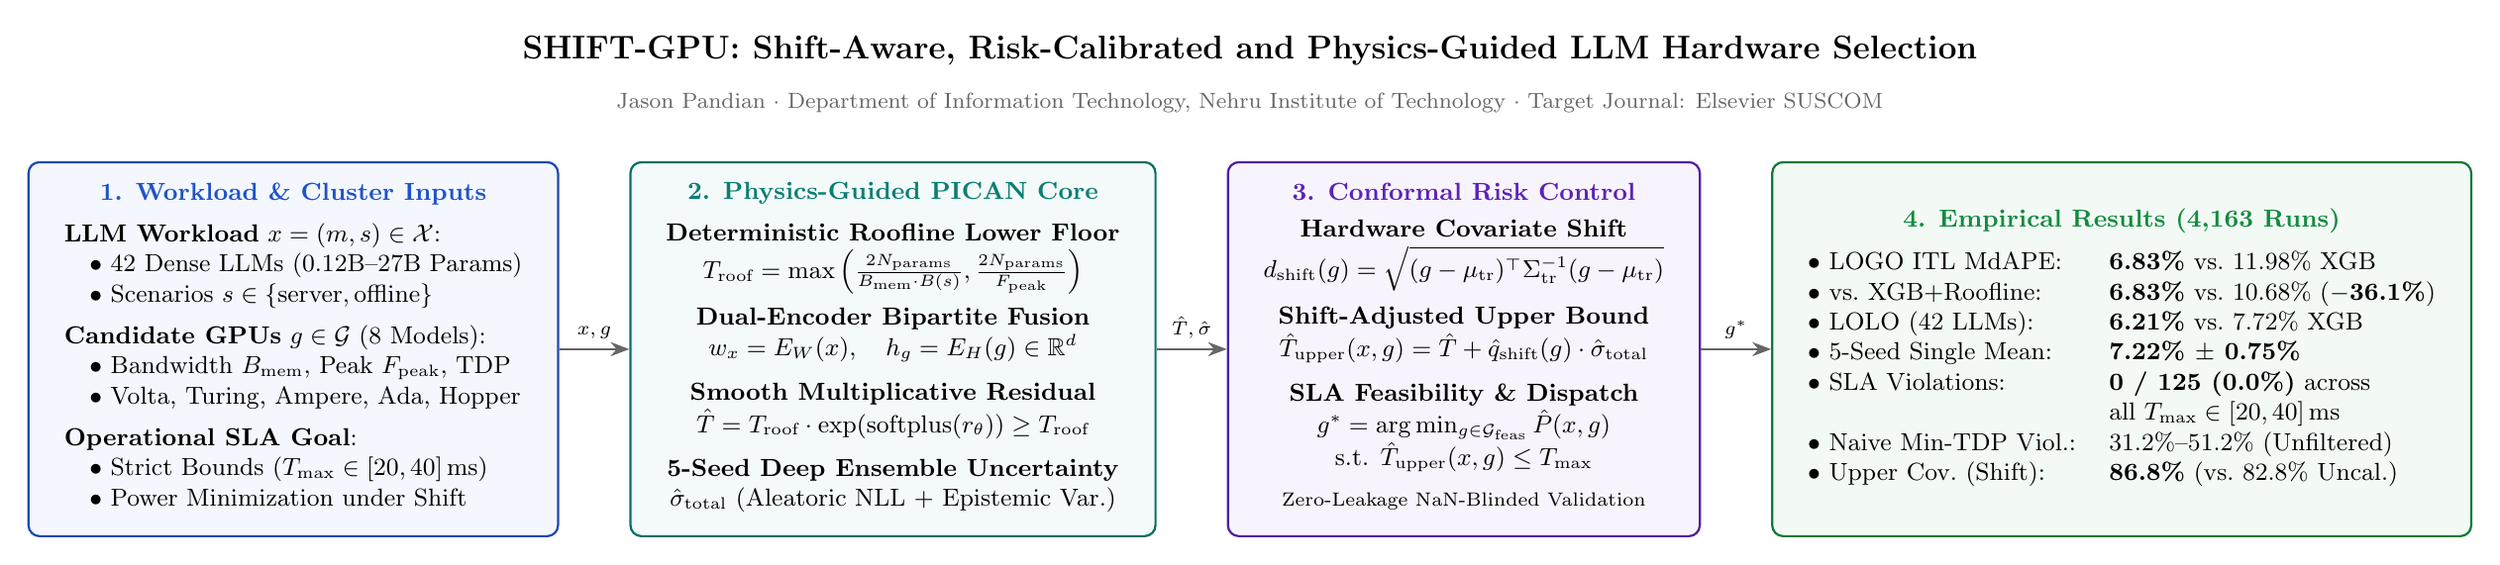
\begin{tikzpicture}[
    auto,
    node distance=0.8cm and 0.9cm,
    card/.style={
        draw=#1!75!black,
        fill=#1!5,
        line width=0.8pt,
        rounded corners=4pt,
        align=center,
        inner sep=7pt,
        font=\small
    },
    arrow/.style={
        -{Stealth[length=2.4mm,width=1.8mm]},
        line width=1.0pt,
        draw=slate!80!black
    }
]
\colorlet{slate}{gray}

% ==================== STAGE 1: INPUTS ====================
\node[card=cblue, minimum width=5.3cm, minimum height=4.8cm] (col1) at (0, 0) {
    {\head{cblue}{1. Workload \& Cluster Inputs}}\\[0.5em]
    \begin{tabular}{l}
    \textbf{LLM Workload} $x = (m, s) \in \mathcal{X}$:\\
    \quad $\bullet$ 42 Dense LLMs (0.12B--27B Params)\\
    \quad $\bullet$ Scenarios $s \in \{\text{server}, \text{offline}\}$\\[0.45em]
    \textbf{Candidate GPUs} $g \in \mathcal{G}$ (8 Models):\\
    \quad $\bullet$ Bandwidth $B_{\text{mem}}$, Peak $F_{\text{peak}}$, $\mathrm{TDP}$\\
    \quad $\bullet$ Volta, Turing, Ampere, Ada, Hopper\\[0.45em]
    \textbf{Operational SLA Goal}:\\
    \quad $\bullet$ Strict Bounds ($T_{\max} \in [20, 40]$\,ms)\\
    \quad $\bullet$ Power Minimization under Shift
    \end{tabular}
};

% ==================== STAGE 2: PICAN CORE ====================
\node[card=cteal, right=0.9cm of col1, minimum width=6.1cm, minimum height=4.8cm] (col2) {
    {\head{cteal}{2. Physics-Guided PICAN Core}}\\[0.5em]
    \begin{tabular}{c}
    \textbf{Deterministic Roofline Lower Floor}\\
    $T_{\text{roof}} = \max\left(\frac{2 N_{\text{params}}}{B_{\text{mem}} \cdot B(s)}, \frac{2 N_{\text{params}}}{F_{\text{peak}}}\right)$\\[0.65em]
    \textbf{Dual-Encoder Bipartite Fusion}\\
    $w_x = E_W(x), \quad h_g = E_H(g) \in \mathbb{R}^d$\\[0.55em]
    \textbf{Smooth Multiplicative Residual}\\
    $\hat{T} = T_{\text{roof}} \cdot \exp(\mathrm{softplus}(r_\theta)) \ge T_{\text{roof}}$\\[0.55em]
    \textbf{5-Seed Deep Ensemble Uncertainty}\\
    $\hat{\sigma}_{\text{total}}$ (Aleatoric NLL + Epistemic Var.)
    \end{tabular}
};

% ==================== STAGE 3: CALIBRATION & SELECTION ====================
\node[card=cpurple, right=0.9cm of col2, minimum width=5.6cm, minimum height=4.8cm] (col3) {
    {\head{cpurple}{3. Conformal Risk Control}}\\[0.5em]
    \begin{tabular}{c}
    \textbf{Hardware Covariate Shift}\\
    $d_{\text{shift}}(g) = \sqrt{(g - \mu_{\text{tr}})^\top \Sigma_{\text{tr}}^{-1} (g - \mu_{\text{tr}})}$\\[0.65em]
    \textbf{Shift-Adjusted Upper Bound}\\
    $\hat{T}_{\text{upper}}(x, g) = \hat{T} + \hat{q}_{\text{shift}}(g) \cdot \hat{\sigma}_{\text{total}}$\\[0.55em]
    \textbf{SLA Feasibility \& Dispatch}\\
    $g^* = \arg\min_{g \in \mathcal{G}_{\text{feas}}} \hat{P}(x, g)$\\
    s.t. $\hat{T}_{\text{upper}}(x, g) \le T_{\max}$\\[0.4em]
    \scriptsize Zero-Leakage NaN-Blinded Validation
    \end{tabular}
};

% ==================== STAGE 4: KEY RESULTS ====================
\node[card=cgreen, right=0.9cm of col3, minimum width=5.3cm, minimum height=4.8cm] (col4) {
    {\head{cgreen}{4. Empirical Results (4,163 Runs)}}\\[0.5em]
    \begin{tabular}{ll}
    $\bullet$ LOGO ITL MdAPE: & \textbf{6.83\%} vs.\ 11.98\% XGB\\
    $\bullet$ vs.\ XGB+Roofline: & \textbf{6.83\%} vs.\ 10.68\% (\textbf{$-$36.1\%})\\
    $\bullet$ LOLO (42 LLMs): & \textbf{6.21\%} vs.\ 7.72\% XGB\\
    $\bullet$ 5-Seed Single Mean: & \textbf{7.22\% $\pm$ 0.75\%}\\
    $\bullet$ SLA Violations: & \textbf{0 / 125 (0.0\%)} across\\
    & all $T_{\max} \in [20, 40]$\,ms\\
    $\bullet$ Naive Min-TDP Viol.: & 31.2\%--51.2\% (Unfiltered)\\
    $\bullet$ Upper Cov.\ (Shift): & \textbf{86.8\%} (vs.\ 82.8\% Uncal.)
    \end{tabular}
};

% Center title cleanly over col1..col4
\path (col1.north west) -- (col4.north east) coordinate[midway] (topmid);
\node[align=center, font=\large\bfseries, anchor=south] (title) at ($(topmid)+(0, 1.1)$)
    {SHIFT-GPU: Shift-Aware, Risk-Calibrated and Physics-Guided LLM Hardware Selection};
\node[align=center, font=\footnotesize, text=gray!80!black, anchor=south] (sub) at ($(topmid)+(0, 0.5)$)
    {Jason Pandian $\cdot$ Department of Information Technology, Nehru Institute of Technology $\cdot$ Target Journal: Elsevier SUSCOM};

% ==================== ARROWS ====================
\draw[arrow] (col1.east) -- (col2.west) node[midway, above, font=\scriptsize\bfseries] {$x, g$};
\draw[arrow] (col2.east) -- (col3.west) node[midway, above, font=\scriptsize\bfseries] {$\hat{T}, \hat{\sigma}$};
\draw[arrow] (col3.east) -- (col4.west) node[midway, above, font=\scriptsize\bfseries] {$g^*$};

\end{tikzpicture}

\end{document}
